\item A small body of mass $m$ tied to a non-stretchable thread moves over a smooth horizontal plane. The other end of the thread is being drawn into a hole $O$ (Fig. 1.49) with a constant velocity. Find the thread tension as a function of the distance $r$ between the body and the hole if at $r = r_0$ the angular velocity of the thread is equal to $\omega_0$.
    \begin{center}
        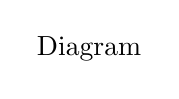
\begin{tikzpicture}
            \node at (0, 0) {Diagram};
        \end{tikzpicture}
    \end{center}\begin{solution}
    \begin{center}
        \begin{tikzpicture}
            \pic at (0, 0) {frame=3cm};
        \end{tikzpicture}
    \end{center}
    
    \begin{align*}
        \intertext{Forces, acting on the mass $m$ are shown in the figure. As $N = mg$, the net torque of these two forces about any fixed point must be equal to zero. Tension $T$, acting on the mass $m$ is a central force, which is always directed towards the centre O. Hence the moment of force $T$ is also zero about the point O and therefore the angular momentum of the particle $m$ is conserved about O.}
        \intertext{So,}
        mr^2\dot{\theta} &= mr_0^2\omega_0\\
        \omega = \dot{\theta} &= \dfrac{\omega_0 r_0^2}{r^2}
        \intertext{From}
        F_r &= ma_r\\
        - T &= m(\ddot{r} - r \dot{\theta}^2)
        \intertext{As the thread is pulled with constant speed so, $\dot{r} = $ constant and $\ddot{r} = 0$ (where dot stands for time derivative).}
        \intertext{Thus}
        T &= F = mr\dot{\theta}^2
        \intertext{Hence, the sought tension is}
        F = mr \dot{\theta}^2 = mr\left(\dfrac{\omega_0 r_0^2}{r^2}\right)^2 &= m\omega_0^2\dfrac{r_0^4}{r^3} \tag{120}
    \end{align*}
\end{solution}